%!TEX root = ../../Compte-rendu.tex
\subsection{Résultats}


\begin{figure}[H]
	\begin{center}
		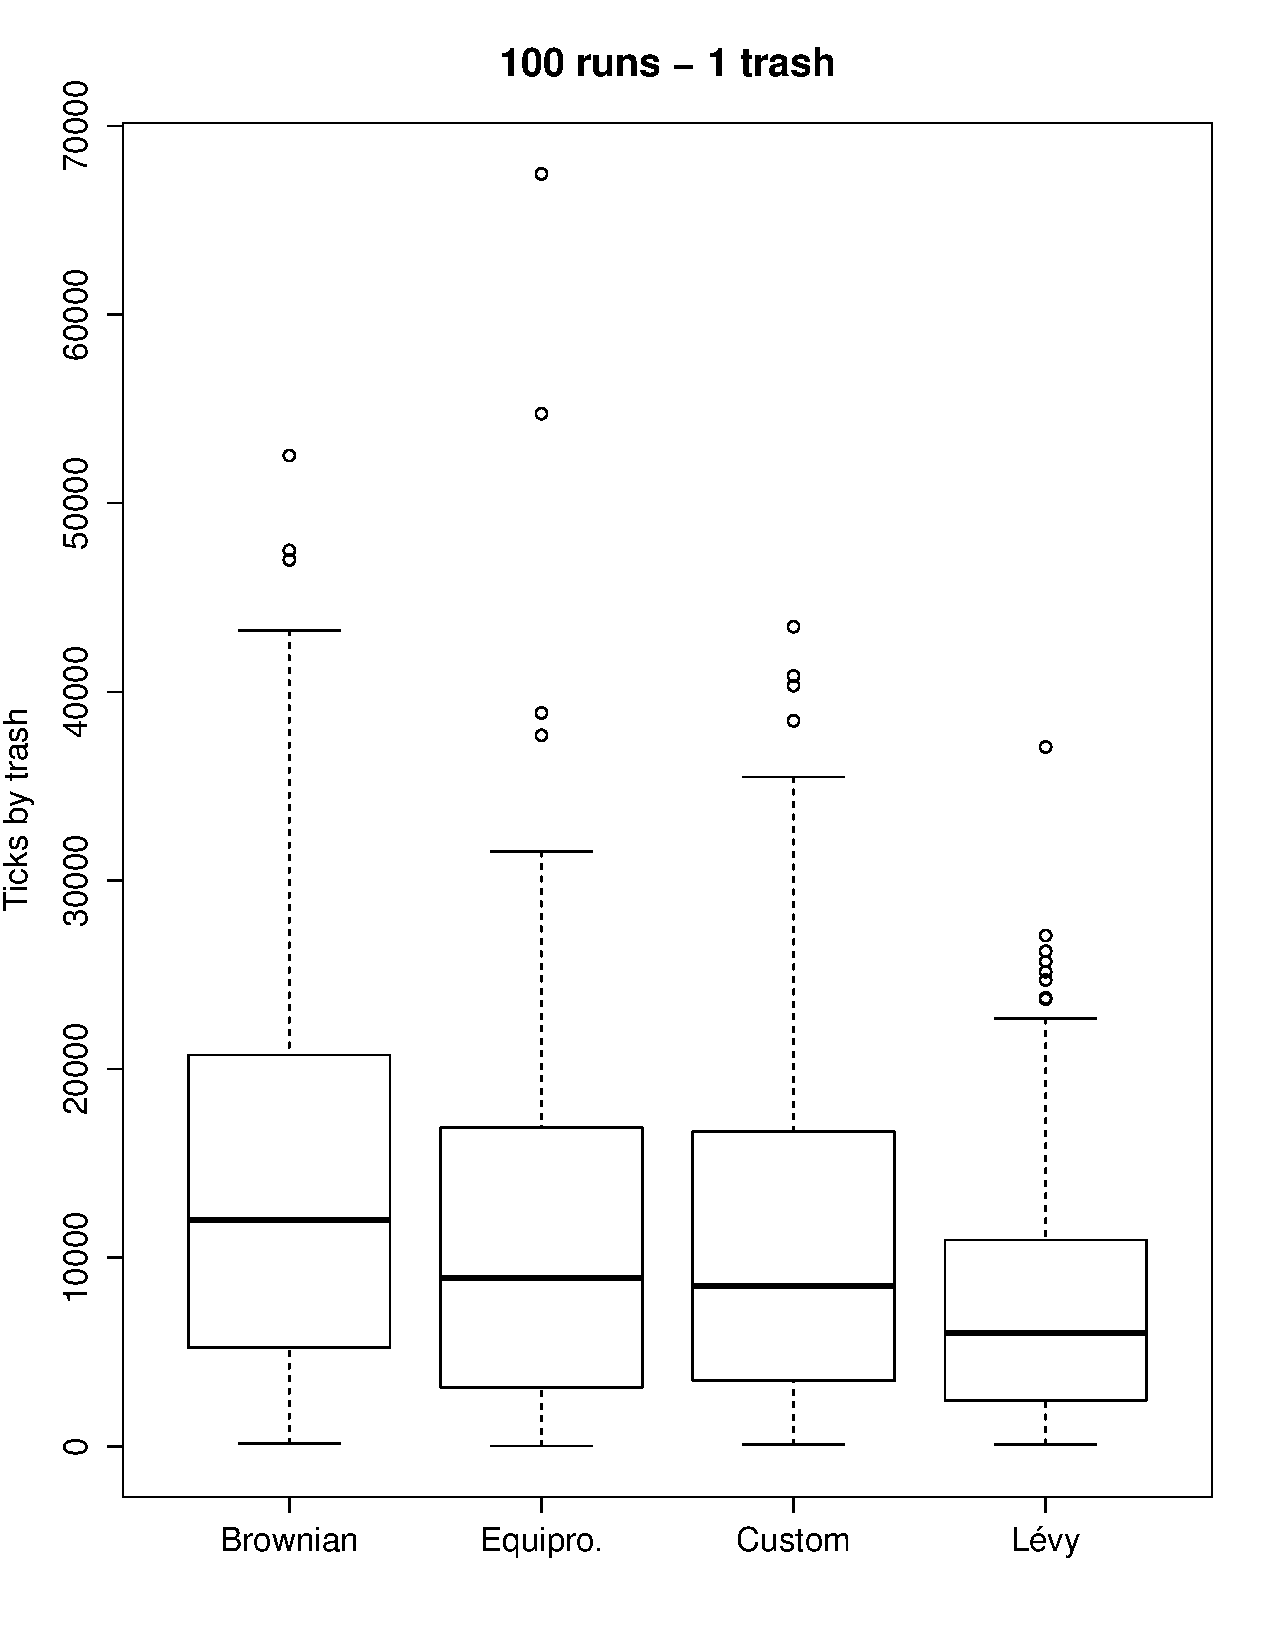
\includegraphics[height=8cm]{diagrams/1Tr_all.pdf}
		\caption{}
		\label{fig:1Trash}
	\end{center}
\end{figure}


Nous avons pour les différentes stratégies les médianes suivantes :

\begin{tabular}{ | c | c | }
	\hline
	\multicolumn{2}{ | c | }{Médianes pour la 1 débris} \\
	\hline
	Brownian & 11981.75 \\
	Equiprobable & 8939 \\
	Custom & 8494 \\
	Lévy & 5994.25 \\
	\hline
\end{tabular}

Nous pouvons voir que les stratégies Equiprobable et Custom sont
équivalentes lorsqu'il est question de trouver un débris unique.


